\documentclass[paperwidth=118cm,paperheight=84cm,portrait,margin=8em,fontscale=0.3]{baposter}
%\usepackage{acl-hlt2011}
%84 cm wide x 118 cm high
\usepackage{times}
\usepackage{svg}
\usepackage{color}
\usepackage{multirow}
\usepackage{latexsym}
\usepackage{amsmath,amssymb}
\usepackage{setspace}
\usepackage{tabularx}

%%30in X 40in
%available sizes: (24 X 38?) (36X48)
%\usepackage{array}
\usepackage{relsize}		% For \smaller
\usepackage{url}			% For \url
\usepackage{epstopdf}	% Included EPS files automatically converted to PDF to include with pdflatex

\newcommand{\compresslist}{
	\setlength{\itemsep}{1pt}
	\setlength{\parskip}{0pt}
	\setlength{\parsep}{0pt}
}
\newenvironment{itquote}
{\begin{quote}\begin{itshape}\begin{small}	\begin{center}\setlength{\parskip}{0.0em}\setlength{\parsep}{0.0em}}
{\end{center}\end{small}\end{itshape}\end{quote}}

\graphicspath{{./}}	% Root directory of the pictures 
\tracingstats=2			% Enabled LaTeX logging with conditionals
%%% Color Definitions %%%%%%%%%%%%%%%%%%%%%%%%%%%%%%%%%%%%%%%%%%%%%%%%%%%%%%%%%

\definecolor{uwPurple}{HTML}{4b2e83}
%\definecolor{uwPurple}{HTML}{3b3e72}
\definecolor{uwGold}{RGB}{232,211,162}
\definecolor{uwMetallicGold}{RGB}{145,123,76}

\begin{document}
\typeout{Poster rendering started}

%%% Setting Background Image %%%%%%%%%%%%%%%%%%%%%%%%%%%%%%%%%%%%%%%%%%%%%%%%%%
\background{
}

\begin{poster}{
	%grid=true,
	columns=3,
	colspacing=2em,
	headerheight = 0.17\textheight ,
	%eyecatcher=false, 
	borderColor=uwMetallicGold,
	headerColorOne=uwPurple,
	headerColorTwo=uwPurple,
	headerFontColor=white,
	% Only simple background color used, no shading, so boxColorTwo isn't necessary
	boxColorOne=white,
	boxColorTwo=uwPurple,
	headerborder=closed,
	headershape=rounded,
	headerfont=\Large\sf\bf,
	textborder=none,
	bgColorOne=uwGold,
	bgColorTwo=uwPurple,
	background=plain,
	headerborder=open,
	boxshade=plain
}
{
%Eye Catcher, empty if option eyecatcher=no
{
	\begin{tabular}{l}
			%
\includegraphics[scale=.6]{graphics/pnt5in.png}
			
\includegraphics[width=2in]{graphics/UWlogo.pdf} \\
			%
\includegraphics[scale=.6]{graphics/pnt5in.png}
			%
\includegraphics[scale=.6]{graphics/pnt5in.png}
	\end{tabular}
	%
\includegraphics[scale=1.7]{graphics/pnt5in.png}
}
}
{ % GUIDE: GUI for Document Exploration
\textbf{Benchmarking Python Deep Learning \\Frameworks on Language Modeling }
}
{
\vspace*{7pt}
\textbf{Lucy Lin, George Mulcaire \& Maarten Sap}\\

%\vspace*{0.5em}
CSE 550 Systems\\
Computer Science and Engineering, University of Washington

 \vspace*{6pt}
}
{
	\begin{tabular}{r}
	
\includegraphics[scale=.6]{graphics/pnt5in.png}
	
\includegraphics[width=1.4in]{graphics/CSElogo.png}
	
\includegraphics[scale=.7]{graphics/pnt5in.png}
	\end{tabular}
}


%For poster contributors, the format is as follows.  Posterboards are 3 feet (90cm) high, 4 feet (120cm) wide self-standing boards that will be placed on top of conference tables. Materials for attaching posters to the boards (double-sided tape, pushpins, clips) will be provided.  Poster authors should finish setting up their posters by the end of the morning break, at the latest.  Also, please note the short "Poster Teasers" in the schedule before the poster session, where you will have 60 seconds (strictly timed!) to give a quick overview that will get people excited about coming to see your poster.
%
%For everyone, please bear in mind that a central goal of the workshop is to create discussion between computational linguists and clinical psychologists.  Therefore we would ask that you please formulate your presentations or posters for a diverse audience, rather than the more typical, purely technical ACL crowd.

%%%%%%%%%%%%%%%%%%%%%%%%%%%%%%%%%%%%%%%%%%%
%%Column 0

%% Box 0
\headerbox{Deep Learning and NLP}{name=intro1,column=0,row=0.00, span=1}{
\color{black}
\vspace*{5pt}
\textbf{Deep learning ``revolution'' in natural language processing}
\begin{itemize}\addtolength{\itemsep}{-0.25\baselineskip}
\item State-of-the-art results are achieved with neural methods \\
(e.g. machine translation, speech recognition)
\item Panoply of toolkits started emerging
\end{itemize}\vspace*{5pt}

\begin{tabular}{ccc}\hspace*{10pt}

\includegraphics[scale=.2]{graphics/pnt5in.png}\\

\includegraphics[width=.24\columnwidth]{graphics/python.jpg}
 & \parbox{0.35\textwidth}{
\vspace*{-40pt}\textbf{Python Frameworks}
\begin{itemize}\addtolength{\itemsep}{-0.5\baselineskip}
\item TensorFlow
\item Theano
\item DyNet
\vspace*{0pt}
\end{itemize}}
& \parbox{0.2\textwidth}{\vspace*{-40pt}

\includegraphics[width=40pt]{graphics/TensorFlow.png}\vspace*{3pt}\\

\includegraphics[width=40pt]{graphics/theano.jpeg}\vspace*{-1pt}\\

\includegraphics[width=40pt]{graphics/DyNet.pdf}
}
\end{tabular}
\begin{center}
\textbf{\textit{Which of these is better when tested on a real NLP task:\\ language modeling?}}
\end{center}
}

%% Box 2
\headerbox{Dataset}{name=intro1,column=0,row=0.415, span=1}{
\color{black}\vspace*{3pt}
English GigaWord corpus (LDC), LA Times from 2009 \vspace*{10pt}
\\
\hspace*{5pt}
\begin{tabular}{cc}
\parbox{0.27\textwidth}{
\vspace*{-0pt}
%
\includegraphics[width=.24\columnwidth]{graphics/newspaper.pdf}
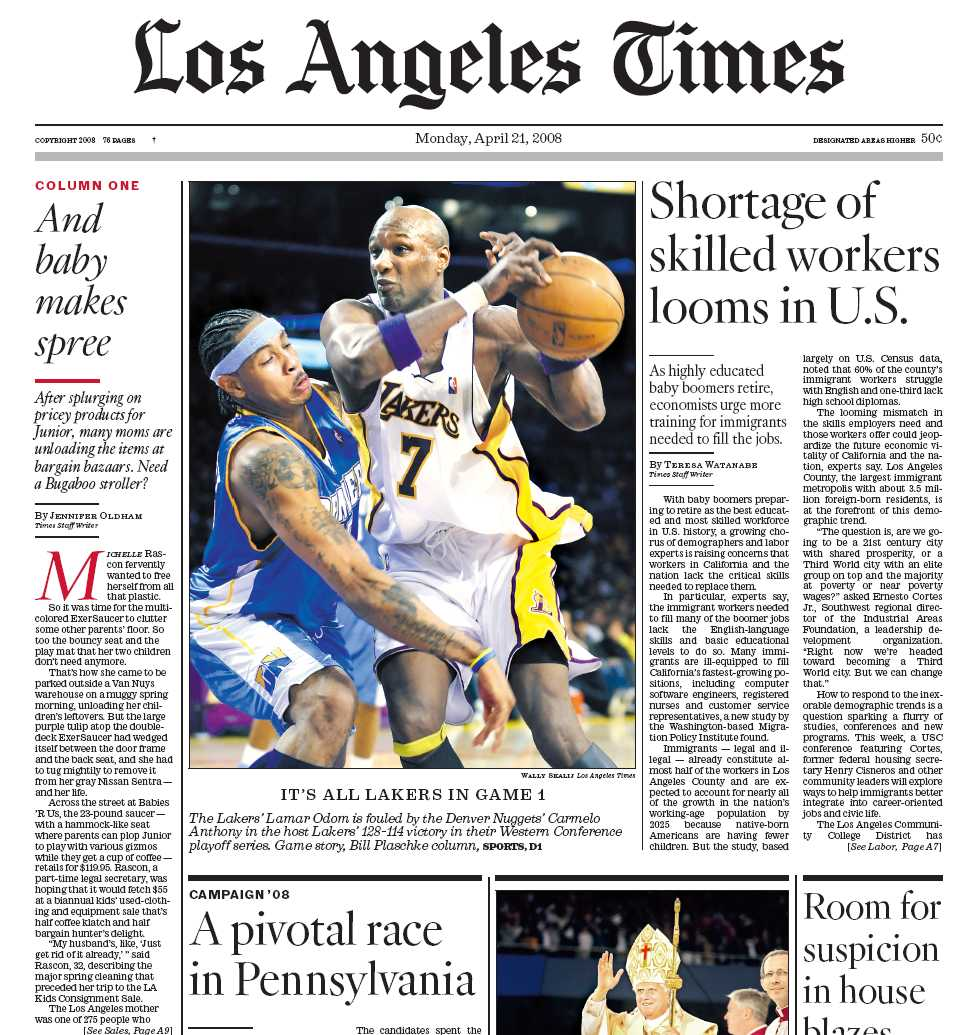
\includegraphics[width=.24\columnwidth]{graphics/latimes.jpg}

}
&
\hspace*{-10pt}
\parbox{0.6\textwidth}{
\textbf{Data}
\begin{itemize}\addtolength{\itemsep}{-0.5\baselineskip}
\item Split into sentences then words \\ using \texttt{NLTK}
\item $1,191,848$ sentences
\item $27,269,856$ words (``tokens'') total
\item $35,642$ distinct words in the end
%\vspace*{-5pt}
\end{itemize}}
\end{tabular}
}

%% Box 2
\headerbox{Model specifics}{name=intro1,column=0,row=0.7, span=1}{
\color{black}
\begin{itemize}\addtolength{\itemsep}{-0.5\baselineskip}
\item Words are embedded in the hidden sized space: $\mathbb{N}^{35642} \rightarrow \mathbb{R}^{256}$.
\item Embedded words are run through the RNN: $w_i = f(w_0^{i-1},\Theta)$.
\item Cross-entropy loss is used to learn the parameters.
\end{itemize}
\begin{center}
\begin{tabular}{cc}
\textbf{hyperparam} & \textbf{value} \\\hline
RNN type & \texttt{LSTM} \\
hidden size & $256$ \\
optimizer & \texttt{AdamOptimizer} \\
learning rate & $0.003$ \\
batch size & 25 \\

\end{tabular}
\end{center}
\vspace{.4pt}
}


%%%%%%%%%%%%%%%%%%%%%%%%%%%%%%%%%%%%%%%%%%%%%%%%%%%%%%%%%%%%%%%%%
%% COLUMN 1

%% BOX 0
\headerbox{Hardware}{name=hardware,column=1,row=0.00,span=1}{
\vspace{0.5em}
\hspace{-15pt}
\begin{tabular}{cc}
\parbox{0.85\textwidth}{
\begin{itemize}\addtolength{\itemsep}{-0.5\baselineskip}
\item \textbf{CPU}: Intel Core i7-5930K, 6 core, 12 thread (3.5 GHz)
\item \textbf{Memory}: G.SKILL Ripjaws 4 Series (8 x 8 GB)
\item \textbf{GPU}: GeForce GTX TITAN X (2 x 12 GB)
\end{itemize}\vspace*{35pt}
} & \hspace*{-10pt}
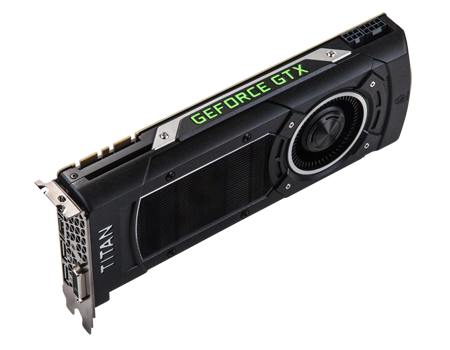
\includegraphics[scale=.1]{graphics/titanx.png}\vspace*{-35pt}
\end{tabular}
% TODO: maybe convert into methodology section -- what experiments we ran (until convergence, single epoch, single batch)
}
\headerbox{Benchmarking strategy}{name=methods,column=1,row=0.1965, span=1}{
\vspace{5pt}
\begin{itemize}
\item \textbf{Timing}: \textit{how long does it take to train/test?}\\ till convergence, single epoch, single batch
\item \textbf{GPU Profiling}: \textit{using the CUDA Profiler}\\overall, matrix multiply, specific GPU metrics
\end{itemize}
\vspace{5pt}
}

\headerbox{Runtime}{name=results,column=1,row=0.415, span=1}{
%
\includegraphics[width=.3\columnwidth]{graphics/TensorFlow.png}
%
\includegraphics[width=.3\columnwidth]{graphics/theano.jpeg}
%
\includegraphics[width=.3\columnwidth]{graphics/DyNet.pdf}

% placeholdering for more appropriate graph
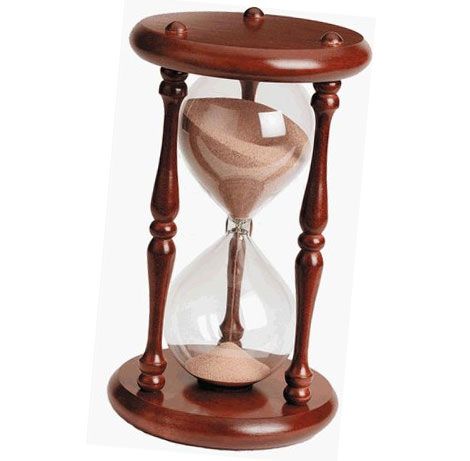
\includegraphics[scale=.07]{graphics/hourglass.jpg}\vspace*{-35pt}
\begin{center}
\textbf{Total runtime on various subtasks, using one GPU:}
\end{center}

\bgroup
\def\arraystretch{1.1}
\setlength\tabcolsep{5mm}
\begin{tabular}{c|ccc}
Time & Dynet & TensorFlow & Theano \\ \hline
Convergence & 26h10m & 35h25m & (TBD)\\
Train epoch & x & 6h57m & 6h35m \\
Test epoch & x & 7m45s & 24m \\
Train batch & 1s & 5s & x \\
Test batch & < 1s & $<$1s & x \\
\end{tabular}
\egroup
\vspace{5pt}
}


%% BOX 1
%\headerbox{Differential Word Clouds}{name=results,column=1,row=0.45, span=1}{
%\begin{center}
%\includegraphics[scale=.5]{graphics/wordcloud1.pdf}
%\includegraphics[scale=.5]{graphics/wordcloud2.pdf}
%\end{center}
%
%Something about the method for creating them ?
%}

%% Box 3
\headerbox{Development experience}{name=methods,column=1,row=0.70, span=1}{
\setlength{\extrarowheight}{3pt}
\begin{tabularx}{\textwidth}{l|X|XX}
\textbf{Framework}  & \textbf{Pros} & \textbf{Cons} \\
\hline
TensorFlow   & Easy to use; good support for RNNs and language models &
    Symbolic computation graph is hard to debug; seems slower than others \\
\hline
Theano  & ``Lower level'' operations $\rightarrow$ highly customizable &
    No built-in support for RNNs (unless using wrapper like Keras)  \\
\hline
DyNet   & Allows flexible models that change during computation & Less documentation and support; fragile dependencies  \\
\end{tabularx}

}


%%%%%%%%%%%%%%%%%%%%%%%%%%%%%%%%%%%%%%%%%%%%%%%%%%%%%%%%%%%%%%%%%
%% COLUMN 2

%% BOX 0
\headerbox{Function-level metrics}{name=results,column=2,row=0, span=1}{
%\begin{itemize}
%\item Time per epoch (for each system)
%\item Time per batch
%\item Most used function/ most resources consumed by (for each system)
%\item Metrics for that function (possibly others that are shared?)
%\item Time to create computation graph
%\end{itemize}

As expected for neural networks, most of the runtime is spent in
matrix multiplication. Focusing on the most frequent function call
(a variant of \texttt{magma\_lds128\_sgemm\_kernel}):

\vspace{1em}

\begin{tabularx}{\textwidth}{l|r}
\textbf{Framework}  & \textbf{Percent time spent in top \texttt{magma\_lds128...}} \\  \hline
TensorFlow  &  68.87\% \\
Theano  & 49.90\% \\
DyNet   & ... \\
\end{tabularx}

\vspace{5mm}

Focusing more closely on this matrix multiply function, we can see how different frameworks make use of the GPU with different levels of efficiency.

\begin{tabularx}{\textwidth}{c|lll}
Metric 										& Dynet & TensorFlow & Theano \\ \hline
\texttt{\detokenize{achieved_occupancy}}			&		.	&		0.062			&		0.062		\\
\texttt{\detokenize{sm_efficiency}}					&		.	&		22.58\%			&		16.04\%		\\
\texttt{\detokenize{warp_efficiency}}					&		.	&		100.0\%			&		99.99\%		\\
\texttt{\detokenize{warp_nonpred_efficiency}}	&		.	&		99.95\%			&		99.91\%		\\
\texttt{\detokenize{global_hit_rate}}					&		.	&		0.00\%			&		0.00\%		\\
\texttt{\detokenize{local_hit_rate}}					&		.	&		0.00\%			&		0.00\%		\\
\texttt{\detokenize{dram_read_throughput}}*		&		.	&		11.07			&		9.97		\\
\texttt{\detokenize{dram_write_throughput}}**		&		.	&		411.99			&		503.54		\\
\end{tabularx}

\vspace{0.5em}
* GB/s \quad ** MB/s
}

%% BOX 1
%\headerbox{Document Viewer}{name=results,column=2,row=0.47, span=1}{
%\begin{center}
%\includegraphics[scale=.4]{graphics/documentView.png}
%\end{center}
%
%The document viewer enables a user to examine a specific text with
%clearly marked frame annotations.
%}

%% BOX 2
\headerbox{Conclusions and Recommendations}{name=results,column=2,row=0.69, span=1}{

}

\end{poster}

\end{document}
